\section{Methodology}
\label{sec:methodology}

\comments{
In this section, we introduce key steps of our works. We first detail how the architecture of SketchPointNet is designed. Next, we will show how to resample each sketch into a fixed number of points. At last, we explain that our group scheme guarantees the integrity of group patterns.}

In this section, we will first introduce the network architecture of our SketchPointNet. Next, we describe the algorithm details of point sampling and grouping from sketch strokes.


\subsection{Architecture of SketchPointNet}
\label{ssec:sketch_point_net}

Fig.~\ref{fig:sketchpointnet} shows the architecture of our SketchPointNet.
%SketchPointNet recognizes sketches as time series. \cxj{Do you input the points as sequence?}
%
\cxj{Why do we need sampling?}.
\wxx{Points from sketches in SVG format are not evenly distributed. They are tend to distribute on the curve strokes. Because curve strokes need more segments to represent. While less points are distributed on the straight strokes. In order to make points evenly distribute on the strokes, we resample the input sketch $\mathcal{S}$ into $N$ points as a point set $\mathbb{P}=\{P_i|i=1,\ldots,N\}$}
The directly captured stroke paths from various input devices are typically contact points that vary largely over different movement speeds and device sizes.
To make them directly comparable, we resample the input sketch $\mathcal{S}$ into $N$ evenly distributed points as a point set $\mathbb{P}=\{P_i|i=1,\ldots,N\}$.
%Moreover, the current Tensorflow only supports static graphs. Resampling the input sketch into a fixed number of points makes the implementation simple.
%
%
\xjmd{Then we extract the sketch features hierarchically with two subnetworks (PN-1 and PN-2).
In each level, we group the sampled point set $\ptset$ into $K$ groups according to their spatial and temporal neighborhoods in different range.
Stroke patterns are extracted using a mini-PointNet~\cite{qi2017pointnetplusplus} for each point group.
}
\cxj{Do you use the same structure as PointNet?}
%
The head of our SketchPointNet is again a PointNet (PN-3) to predict the probability for the $K$ categories with a soft-max\cxj{predict the probability for the $K$ categories with a soft-max?}.



While the overall architecture of our SketchPointNet is similar with PointNet++~\cite{qi2017pointnetplusplus}, the main difference lies on the sampling and grouping procedure.
Targeting at 3D point clouds, PointNet++~\cite{qi2017pointnetplusplus} considers the spatial distribution of points in the 3D space.
In contrast, not only the spatial pattern is important, the temporal pattern is also important for sketch recognition.
%
During our sampling and grouping, the temporal and spatial information is integrated together to extract the sketch pattern.

\subsection{Transform Network}
\cxj{Add more details. }

\wxx{We predict an affine transformation matrix by a T-net and affine transformation matrix on the input points. This step make sure that input sketches are spatially transformed and aligned.}


\subsection{Sketch Sampling}
\label{ssec:resample}

%% key concept of resampling�� preserve local temporal and spatial relations��
To preserve the sketch pattern xxxx
sample various input sketches into a fixed number points,
%
Therefore, we sample $N_{pt}$ equidistantly spaced points along strokes.
%
We calculate the length of each stroke and the total length of all strokes is $L_{sum}=\sum^{M}_{i=1} L_i$, where $M$ is the stroke number.
%
Given the desired point number $N_{pt}$, we assign each stroke $N_i=\frac{L_i}{L_{sum}}N_{pt}$ points according to its stroke length $L_i$.
Then we reample each stroke into $B_i$ points equidistantly along the stroke.
%
Fig.~\ref{fig:resample} shows the sampling results with different number of points.
\xjmd{We can see that the main structure is well preserved during the resampling procedure without losing much details, even with a very small number (N=128) of points.}


\begin{figure}
	\center
	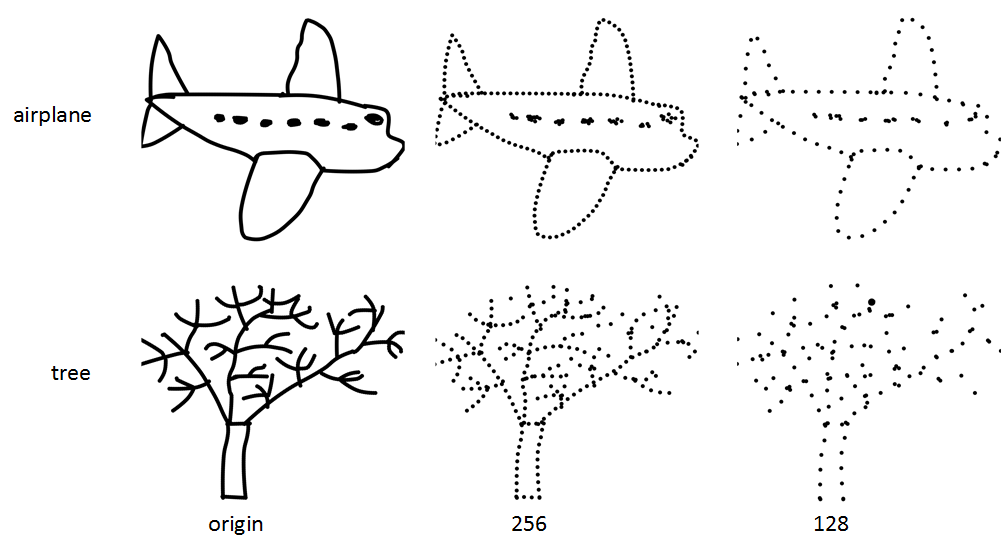
\includegraphics[width=3in]{images/resample2.png}
	\fcaption{Sketch resampling with different number of points. \cxj{Show different stroke in different color?}}
	\label{fig:resample}
\end{figure}



\subsection{Point Grouping}
\label{ssec:group_scheme}

\xjmd{To extract local features of the input sketch, we group the sampled points and feed them into a PointNet.}
%
Given a desired number of groups $N_{group}$, we first sample $N_{group}$ points as the group centers from the input sketch \wxx{from the input $N$ points with a fixed interval} \cxj{using the same resample method in Sec.~\ref{ssec:resample}?}
%
Then we extract the local feature for each group from the points in a its surrounding area in a radius $r$.
%
While the sketch is resampled evenly distributed temporarily in the previous sampling step, the point density is not even in the spatial
domain.
%
We resample the partial sketch in a local region to a fixed number $K_{group}$ of points equidistantly.
%
As Fig.~\ref{fig:group} shows, the points in a local region
with different radius present different local patterns.
Both temporal and spatial patterns are preserved during the grouping procedure, which are essential for sketch recognition.




\subsection{Group Pattern Extraction}

We use the PointNet~\cite{qi2017pointnet} to extract the sketch pattern in a local region that contains a flexible number of points.
%
%After the point grouping step, we feed a mini PointNet with $N_g$ groups with data size $N_g \times K_g \times C$ to extract the sketch pattern for recognition.
%
For each group, a mini PointNet is fed with $K_g$ points in its local region with data size $K_g \times C_{in}$.
Here, $K_g$ is the number of points in a group, and $C$ is the number of data channel of each point.
Each mini PointNet consists of $K_g$ shared-weight three-layer perceptrons and a max-pooling layer to aggregate features of the $K_g$ points.
%
The output of the a PointNet is a $C_{out}$ dimensional feature vector.
%Here, $N_g$ is the number of local groups, $K_g$ is the number of points in each group, $C$ is the number of data channel of each point.

Initially, we have the 2{D} coordinates and stroke order of each point.
We translate each point into a local frame relative to the group center of each group.
Therefore, the data channel $C^1_{in}=2+1$ for the first PointNet PN-1, including the 2D local coordinates and 1-D stroke order.
The output of PN-1 is a $C^1_{out}$ dimensional feature vector for each group.

%
%
Different with PointNet++~\cite{qi2017pointnetplusplus} for 3D point clouds, the stroke order does matters for sketch recognition, because human typically draw the overall shape and then add fine details later.
%
The strokes drawn earlier have more impact effects for recognizing a coarse sketch.
%

Then, increasing the radius $r_2$ for grouping points, which is equivalent to increasing the receptive field, we extract sketch patterns in a higher level.
%
Therefore, for the second PointNet PN-2, the input is the $K_{g2} \times C^2_{in}$ data, where $K_{g2}$ is the number of points in the local region of a group, $C^2_{in}=2+1+C^1_{out}$ for each group, including the 2-D local coordinate of the group center, 1-D stroke order and the $C^1_{out}$-D feature extracted for the local region from the first PointNet.
%
The output of PN-2 is a $C^2_{out}$-D feature vector for each group.

\subsection{Sketch Classification}
\label{ssec:classification}

After the two-level local pattern extraction, we feed the $N_{g2} \times C^2_{out}$ data into the third mini PointNet PN-3, which produces $C^{3}_{out}$ dimensional vector as the global feature of the entire sketch.
%
\cxj{More details about the FC layers and loss functions.}
The extracted global feature is fed into a four-layer perceptron to predict the scores for $K_c$ categories.
\wxx{Then we calculate $K_c$ softmax scores from predicted scores. With cross softmax scores, we use cross entropy as our loss function.}







\begin{figure}
    \center
    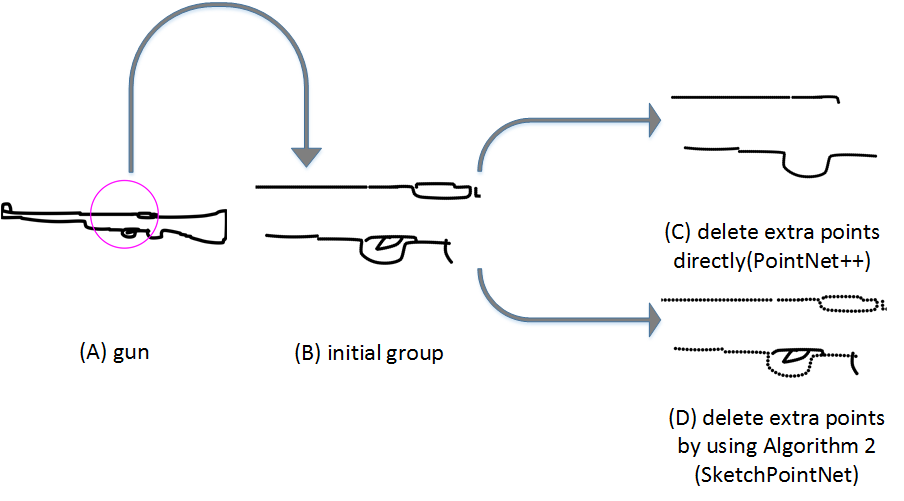
\includegraphics[width=3in]{images/group.png}
    \fcaption{Comparison of dealing with extra points.}
    \label{fig:group}
\end{figure}